\clearpage
\section{Research topics to be investigated}
\label{ch:proposal}

This section presents some main ideas for the continuity of this doctoral
research project. \autoref{sec:topics} brings the research topics to be
addressed while \autoref{sec:timetable} shows the work plan and timetable.

%=============================================================================%
\subsection{Research topics}
\label{sec:topics}

The research topics to be addressed are divided into three topics, which are
detailed in Sections~\ref{subsec:distributed} through \ref{subsec:handover}.
Each topic encompasses the motivation, goals, and objectives.

%-----------------------------------------------------------------------------%
\subsubsection{Scalable controller architecture}
\label{subsec:}

Este projeto tem como objetivo projetar uma entrega de vídeo baseada em DASH confiável e de alta qualidade para ser usada em ambientes de cidades inteligentes~\cite{gamaUCC2019, KreuzbergerWorkshop2016}. O esquema proposto aproveitará várias tecnologias relacionadas à rede, como Cloud, Fog e Edge Computing, além de posicionamento e encadeamento inteligente de serviços.% A Figura~\ref{fig:scenario-arch} descreve, no lado esquerdo, uma arquitetura de rede de várias camadas, composta por um conjunto heterogêneo de dispositivos e aplicativos que utilizam recursos de computação distribuídos por meio de uma tecnologia de comunicação de acesso múltiplo, como 5G e WiFi. Este projeto propõe estender o streaming de vídeo DASH para suportar conectividade simultânea de caminhos múltiplos~\cite{poliakovPHD2018, Velasquez2018}.

%O lado direito da Figura~\ref{fig:scenario-arch} descreve parte dos parâmetros que devem ser avaliados para definir quais serviços de vídeo precisam ser implantados, juntamente com a camada mais adequada para implantar cada um deles. Observe que os parâmetros na camada mais inferior para feedback diferem dos de outras camadas. Inicialmente, os parâmetros avaliados considerados incluem o perfil do usuário, a carga da célula local, a qualidade do link, a complexidade do movimento dos vídeos e também detalhes inteligentes da cidade, como a localização e a rota rastreada no caso de usuários com mobilidade. Alguns dos nós podem ser estacionários, mas outros podem variar de padrões de baixa a alta mobilidade, que podem ser levados em consideração para melhorar a qualidade da entrega de vídeo.

\vspace{0.8cm}
\begin{figure*}[htpb]
	\centering
	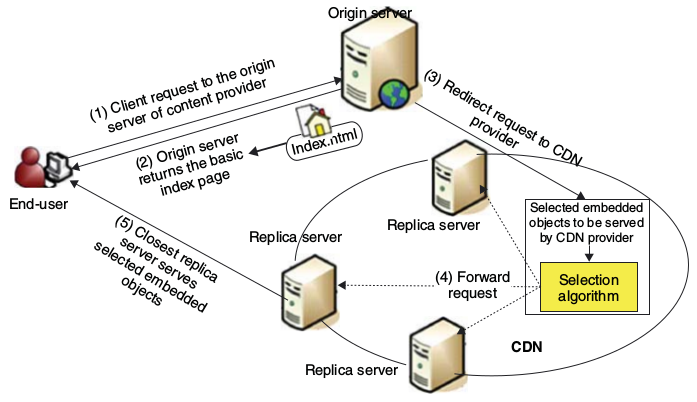
\includegraphics[width=0.7\textwidth]{img/fig-intro.png}
% 	\vspace{-1cm}
	\caption{DASH-based Adaptive Multimedia Delivery System for Cloud/Fog Nodes.}
	\label{fig:scenario-arch}
\end{figure*}

Dada a arquitetura do modelo de serviço e ambiente de nuvem/borda de várias camadas mencionada, este trabalho tem como objetivo abordar algumas das seguintes questões de pesquisa:~\textit{i)} Como determinar as melhores camadas para alocação de serviços de vídeo?~\textit{ii)} Como os pedaços de vídeo não solicitados devem ser distribuídos na hierarquia de borda/nuvem, considerando as informações de localização do usuário e estimativas sobre a localização futura do usuário em tempo real?~\textit{iii)} Como facilitar o streaming de vídeo através de várias fontes simultaneamente?~\textit{iv)} Como os algoritmos de adaptação à taxa de bits podem ser afetados pelo tamanho do pedaço de vídeo em uma arquitetura de várias camadas?

\subsection{Multimedia Delivery System Schemes}
% Selection Algorithms

\subsection{Game Theory Based Adaptative Bit Rate Scheme}

% This project aims to design a reliable and high-quality DASH-based video delivery to be used in Smart City Environments~\cite{gamaUCC2019, KreuzbergerWorkshop2016}. The proposed scheme will take advantage of several network-related technologies such as Cloud, Fog, and Edge Computing, as well as intelligent service placement and chaining. Figure~\ref{fig:scenario-arch} depicts, on its left-hand side, a multi-tier network architecture, which is composed of a heterogeneous set of devices and applications using distributed computing resources through a multi-access communication technology, such as 5G and WiFi. This project proposes to extend DASH video streaming to support simultaneous multipath connectivity~\cite{poliakovPHD2018, Velasquez2018}.

% The right-hand side of Figure~\ref{fig:scenario-arch} describes part of the parameters that should be assessed to define which video services are needed to be deployed along with the most suitable tier to deploy each of them. Note that the parameters in the bottommost tier for feedback differ from those of other tiers. Initially, the assessed parameters considered include the user's profile, the load of the local cell, the link quality, the motion complexity of the videos, and also smart city details such as the location and the traced route in case of users with mobility. Some of the nodes can be stationary, but others can range from low to high mobility patterns, which can be taken into account to improve quality of video delivery.

% \vspace{0.8cm}
% \begin{figure*}[htpb]
% 	\centering
% 	\includegraphics[width=1.0\textwidth]{images/scenario_incomplete}
% % 	\vspace{-1cm}
% 	\caption{DASH-based Adaptive Multimedia Delivery System in an Smart City Environment.}
% 	\label{fig:scenario-arch}
% \end{figure*}

% Given the aforementioned multi-tier edge/cloud environment and service model architecture, this work aims to tackle some of the following research questions:~\textit{i)} How to determine the best tiers for video services placement?~\textit{ii)} How unsolicited video chunks should be distributed in the edge/cloud hierarchy considering user location information and estimates on future user location in real time? ~\textit{iii)} How to facilitate video streaming through multiple sources concurrently?~\textit{iv)} How bitrate adaptation algorithms can be impacted by video chunk size in a multi-tiered architecture?


% Neste trabalho, queremos construir um sistema CDN na fog com o uso de cache e sobreposição de rede para para streaming de video ao vivo, e otimizar sua topologia de forma adaptativa para minimizar a latência de reprodução média e melhorar a entrega do fluxo de forma oportuna. A latência de reprodução é a diferença entre o tempo de reprodução (ponto de reprodução) na origem de mídia e em um nó.

% \vspace{1cm}
% \noindent
% \textbf{Modelagem de propriedades de balanceamento de carga e desempenho de cache em sistemas de Névoa-Nuvem multicamadas.}

%-----------------------------------------------------------------------------%
\subsection{Medidas objetivas}


%-----------------------------------------------------------------------------%
\subsubsection{Scalable controller architecture}
\label{subsec:distributed}

Having a centralized controller is by no means an intrinsic characteristic of
\ac{SDN}. According to \citet{Kuklinski2014a}, there are obvious benefits on
the \ac{SDN} centralized network control approach, but the controller appears
to be a single point of failure and scalability, which raises potential
performance issues of the control plane in terms of reaction time or volume of
control traffic. As indicated by \citet{Yeganeh2013}, the central controller
does not scale as the network grows (increase the number of switches, flows,
bandwidth, etc.) and will fail to handle all the incoming requests while
providing the same service guarantees.

Previous research into improving \ac{SDN} scalability are categorized into
three groups by \citet{Sato2015}: (1) improving the performance of the
controller itself, (2) reducing the workload of the controller, (3) and
designing a distributed architecture for the control plane. The first group is
related to hardware and software improvements, like multi-threads applications
over dedicated hardware. It is possible to reduce the workload of the
controller by extending the functionality of switches on the data plane. Using
pre-installed rules, dividing data flows into classes, and installing
aggregated matches are examples of improvements in this second group. Finally,
the third group includes new control plane architectures, increasing the number
of \ac{SDN} controllers in the management domain.

\citet{Arslan2015} discuss this distributed architecture for the control plane.
There is a propensity to develop new \ac{SDN}-based architectures that are
scalable through the hierarchy of controllers. The most efficient management
approach seems to be hierarchical one in which the network, for the management
purposes, can be split into smaller geographical domains that are locally
managed and coordinated by a network management center~\cite{Kuklinski2014a}.

As depicted in \autoref{fig:centralized-controller}, the current centralized
\ac{EPC} controller architecture introduced in \autoref{sec:controller} has a
single controller element that is responsible for traffic routing, bearer
admission control, and \ac{QoS} realization. This single entity manages all
switches in the infrastructure layer using the OpenFlow southbound interface.
Also, it communicates with the \ac{MME} element over a non-standardized
northbound interface.
\begin{figure}[htb]
  \centering
  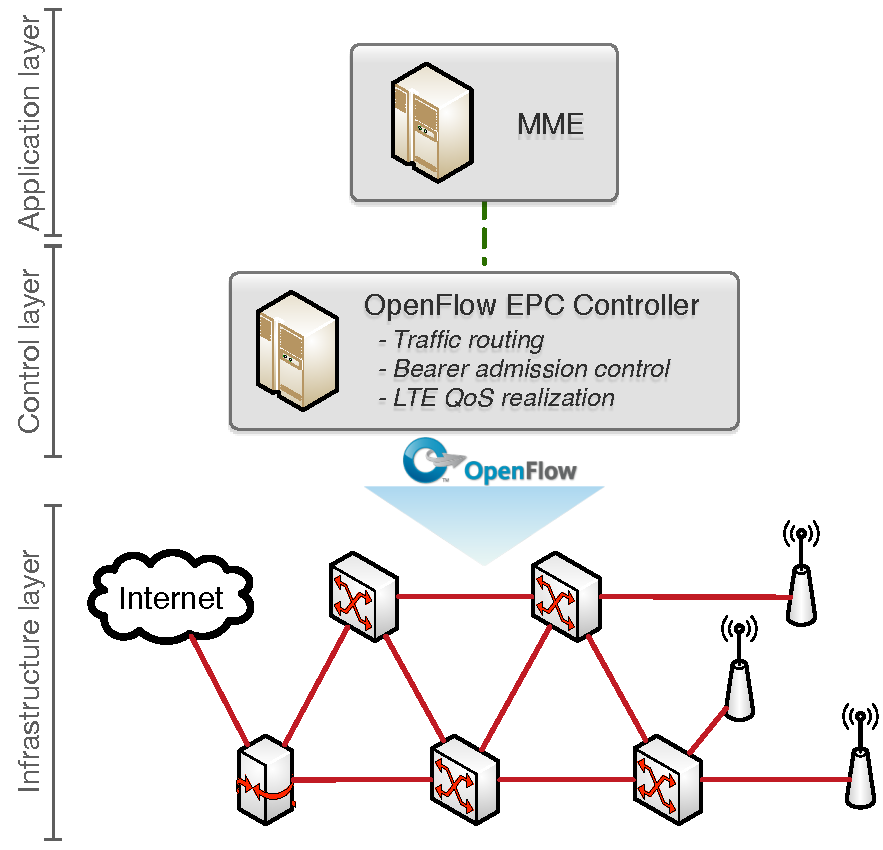
\includegraphics[scale=0.5]{centralized-controller}
  \caption{The current centralized \acs{EPC} controller architecture.}
  \label{fig:centralized-controller}
\end{figure}
This centralization issue can be partially solved by splitting the network into
smaller domains. As nodes in mobile networks are usually geographically
distributed, \citet{Yeganeh2013} say that it is possible to take advantage of
the physical distribution of the network to partition it into separate regions;
each partition can be controlled by an independent controller, and these
controllers can exchange only the required state changing events, effectively
hiding most events from external controllers. \citet{Yang2015a} say that there
is no need to provide a strictly consistent centralized view to each
controller, which would cause processing overload and additional cost when the
network expands.

\emph{The goal of this research topic is} to improve the current controller
model toward a scalable architecture. \autoref{fig:distributed-controller}
shows a possible distributed \ac{EPC} controller architecture, where the
\acp{eNB} are enhanced with a local controller and switch that are used for
traffic classification purposes at the network edge. A centralized topology
controller can independently handle topology-related questions (like traffic
routing) in the backhaul network. Finally, a specialized \ac{QoS} controller
would be in charge of admission control and \ac{QoS} management, communicating
with edge and topology controller. Theses controllers can be assisted by
applications, like network mapper and routing and a more sophisticated
admission control software. 
\emph{The objectives for this research topic are:}
\begin{itemize}
  \item Determine the controller functionalities that can be performed
  independently of each other, to effectively proposed a distributed controller
  architecture;

  \item Model the inter-controller communication for the distributed controller
  architecture, reducing the amount of information exchanged between
  controllers;

  \item Evaluate possible standardized east/westbound interfaces for controller
  interaction;

  \item Implement and evaluate the proposed architecture in the \ac{ns-3}
  simulator, performing scalability tests with large numbers of \acp{eNB} and
  \acp{UE} in the network.
\end{itemize}

\begin{figure}[htb]
  \centering
  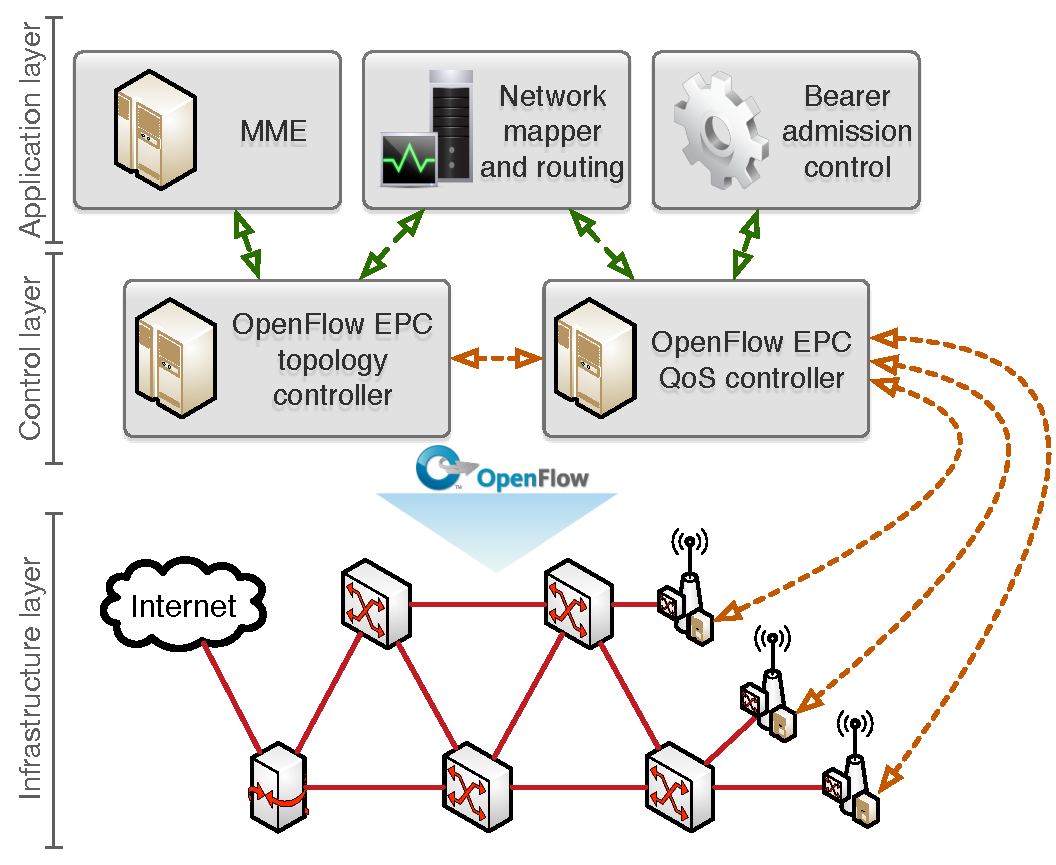
\includegraphics[scale=0.5]{distributed-controller}
  \caption{A possible distributed \acs{EPC} controller architecture.}
  \label{fig:distributed-controller}
\end{figure}

%-----------------------------------------------------------------------------%
\subsubsection{Traffic offloading in \acsp{HetNet}}
\label{subsec:heterogeneous}

As the wireless link efficiency is approaching its fundamental limits, further
improvements in cellular system spectral efficiency are only possible by
increasing the node deployment density. As observed by \citet{Damnjanovic2011},
challenges associated with the deployment of traditional macro base stations
can be overcome by the utilization of base stations with lower transmit power.
A network that consists of a mix of macro cells and low-power nodes, where some
may be configured with restricted access and some may lack wired backhaul, is
referred to as a \acf{HetNet}. \autoref{fig:hetnet} exemplifies a \ac{HetNet}
with a macro cell, some metro and picocells used for relay, some network
operator deployed low-costs indoor and outdoor small cells, and user deployed
very low costs for indoor environment.

\begin{figure}[htb]
  \centering
  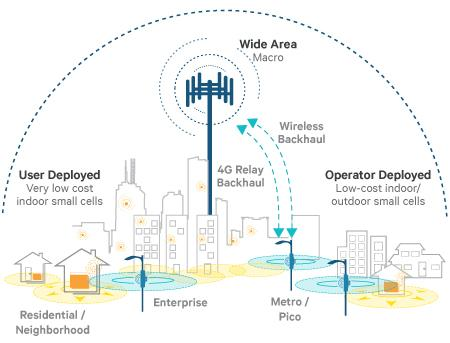
\includegraphics[scale=0.55]{hetnet}
  \caption{A \acs{HetNet} example scenario~\cite{Qualcomm2014}.}
  \label{fig:hetnet}
\end{figure}

The future 5G architecture must provide a communication environment able to
overcome the infrastructure shortcomings of current networks. Networks will
become much denser with many more cells with decreasing size as well as direct
device-to-device communication. Small cells improve capacity and cellular
coverage with lower cost compared to macrocells, and they are expected to carry
the majority of traffic. \citet{Pierucci2015} says that while bringing the base
station closer to the user, it is possible to promote lower power use and more
energy efficient communications. In the opinion of \citet{Einsiedler2015}, the
vision is to provide functional convergence of network control to handle 5G,
4G, older access technologies, and Wi-Fi; enabling a flexible and efficient
support and deliver all types of applications.

As claimed by \citet{Tomici2015}, network operators have shown more interest in
deploying integrated small cell and Wi-Fi accessing networks to accommodate the
increasing demand for bandwidth caused by widespread wireless data usage.
However, the 3GPP interworking architecture forces the inter-system handover to
happen solely at the \ac{P-GW}, which may cause unnecessary burdens on the
mobile core network, especially with the expected large number of small cell
and Wi-Fi accessing network deployment.

Within an \ac{SDN} architecture, the user data plane can be distributed to
allow local offloading of user data traffic, regulated by the (partially)
logically centralized network controller. An example of traffic offloading
solution is the one proposed by \citet{Ghazisaeedi2013}, where a switching
system is used to redirect \ac{HTTP} traffic from \ac{S-GW} to the Internet.
This technique can decrease the traffic load over the mobile core network. In
\citet{Tomici2015}, the authors suggest three new \ac{LTE}-\ac{WLAN}
integration architectures for inter-system handover, which are based on having
a local integration point. For each of these integrated architectures, the
authors propose a network-initiated inter-system handover mechanism between the
\ac{eNB} and \ac{WLAN} \ac{AP}. The handover mechanisms are efficient due to
limited interaction with the \ac{P-GW} in the core network.

\emph{The goal of this research topic is} to design an algorithm responsible
for offloading \ac{LTE} traffic over available Wi-Fi networks. Assuming that
many Wi-Fi hotspots are deployed by the mobile operators in public urban areas,
the algorithm focus is to trigger offloading decisions based on the current
traffic load in the backhaul and core networks.
\emph{The objectives for this research topic are:}
\begin{itemize}
  \item Compare current approaches for traffic offloading in mobile networks,
  identifying the benefits and drawbacks of each solution;

  \item Propose an improved offloading decision solution for \ac{EPC}, using
  Wi-Fi as enabler technology;

  \item Implement and evaluate the proposed solutions in the \ac{ns-3}
  simulator, performing tests on scenarios with different access networks.
\end{itemize}

%-----------------------------------------------------------------------------%
\subsubsection{Distributed mobility management}
\label{subsec:handover}

Mobility management refers to a set of mechanisms to keep ongoing sessions
continuity while a mobile user changes its mobility anchor point in the
network. In the \ac{LTE} architecture, mobility management solutions rely on
centralized mobility anchor entities (\ac{S-GW} and \ac{P-GW}), which are in
charge of both mobility-related control plane and user data forwarding.
According to \citet{Valtulina2014}, this centralized approach makes mobility
management prone to several performance limitations such as suboptimal
routing, low scalability, potential single point of failure and the lack of
granularity for the mobility management service.

Nowadays, \acf{DMM} is considered as a promising solution to solve these above
challenges. Several proposals tried to redesign mobile network architecture by
leveraging \ac{SDN} and OpenFlow with the support of \ac{DMM}.
\citet{Karimzadeh2014} discuss the \ac{DMM} in \ac{LTE} systems composed of
virtual gateways running on the cloud. \citet{Kuklinski2014b} discuss the
evolution of mobility management mechanisms in mobile networks and how \ac{SDN}
can be applied to efficiently handle mobility in the context of future 5G
networks. In the CROWD architecture~\cite{Ahmad2013a}, a \ac{DMM} gateway
replaces current anchor points, and mobility management functions are executed
by control applications. \citet{Gurusanthosh2013} propose the \acf{SDMA} in
\ac{LTE} backhaul access networks, including detailed handover procedure with
dynamic anchor element choice, which is based on \ac{UE} location and path
changes during handover. \citet{Mahmoodi2014} introduce a distributed \ac{SDN}
control plane with mobility management as an example where the controller
becomes responsible for handover procedures, reducing the power consumption of
the \ac{UE} and the signaling message overhead between entities at the backhaul
side.

Besides, mobility management may no longer be exclusively triggered by radio
quality, but also by network management decisions~\cite{Rost2014}. Several
redesigned handover procedures are proposed by \citet{Zhang2015b} for 5G ultra
dense networks. They take advantage of control and user-plane separation,
taking into consideration of mobility, stability, energy efficiency and
realizability.

Particularly, handover performance can severely impact the \ac{QoS} in
\acp{HetNet}. The increasing number of small nodes bring cells closer and there
is no more obvious boundary between them, enhancing the capacity per area by
the space division multiplexing. \citet{Sun2015} propose intelligent schemes
to handle the dynamic environment of \acp{HetNet}. The authors identify some
key problems in 5G \acp{HetNet} as traffic control, load balancing, density
prediction, and resource allocation. Then, they develop a number of smart
schemes to overcome these challenges.

\emph{The goal of this research topic is} to distribute the mobility management
computation intensive task among the \ac{MME} and a number of controllers nodes
in the network, avoiding a centralized operation. The handover processing can
also be assisted by a sophisticated software application. With this approach,
it is possible to reduce signaling overhead over backhaul and core network and
speed up handover procedures. The development of such distributed solution will
be guided by group handover in heterogeneous environments, when a group of
users may change the access networks simultaneously or within short
time~\cite{Chowdhury2012}.

Another opportunity is to explore \ac{SDN} flexibility and move the anchor
point to the OpenFlow backhaul network, considering that when a \ac{UE} is
handed over to a new access point, in most cases a large part of the path that
the traffic takes in the backhaul network would be the same before and after
the handover. \autoref{fig:lte-handover} shows how \ac{GTP} tunnels are handled
during a normal handover procedure in \ac{LTE} networks, and
\autoref{fig:dmm-proposal} exemplifies how the proposed distributed mobility
management solution can handle the \ac{GTP} tunnels, following some ideas from
the \ac{SDMA}. Nonetheless, while \ac{SDMA} demands changes in the standard
procedures with no backward compatibility, the proposed solution must be
designed to offer interoperability with existing networks.

\begin{figure}[htb]
  \centering
    \subfloat[Centralized anchor.]
    {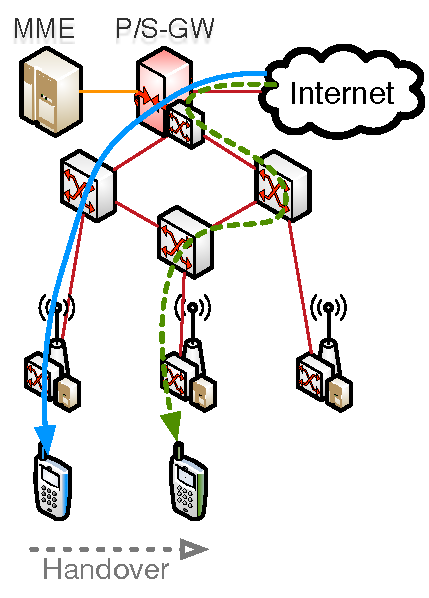
\includegraphics[width=.25\textwidth]{lte-handover}
    \label{fig:lte-handover}}
  \hfil \hspace{1cm}
    \subfloat[Distributed anchor.]
    {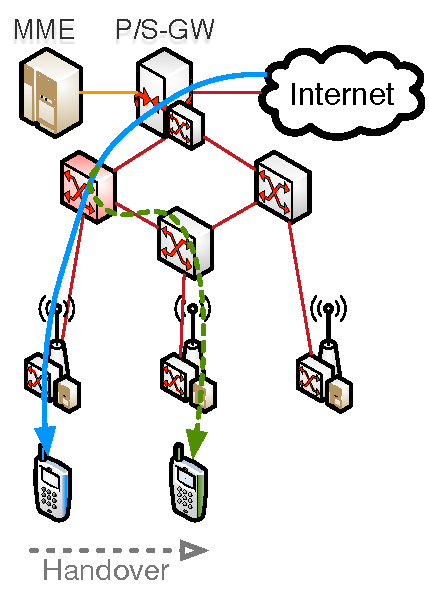
\includegraphics[width=.25\textwidth]{dmm-proposal}
    \label{fig:dmm-proposal}}
  \caption{\acs{SDN}-enabled \acs{LTE} network topology.}
  \label{fig:dmm}
\end{figure}

\emph{The objectives for this research topic are:}
\begin{itemize}
  \item Detailed study of \ac{LTE} handover procedures to propose a suitable
  distribution among \ac{MME} and available OpenFlow controllers, considering
  the interoperability with \ac{3GPP} standards;

  \item Examine available solutions for load balancing in mobile networks,
  which can be used to trigger handover procedures in the distributed
  architecture;

  \item Analyze existing solutions for vertical handover in \acp{HetNet},
  taking care of handovers between overlapping macro and small cells;

  \item Assess approaches for rerouting tunnels in OpenFlow backhaul network,
  looking for an optimal anchor element;

  \item Implement and evaluate the proposed \ac{DMM} in the \ac{ns-3}
  simulator, performing handover tests with groups of \acp{UE} between
  \acp{eNB}.
\end{itemize}


%=============================================================================%
\subsection{Work plan and timetable}
\label{sec:timetable}

\autoref{tab:timetable} presents the timetable for this doctoral research
project. The activities referenced in the timetable are listed below and
comprises both the developed work introduced in \autoref{ch:developed} and the
topics to be investigated from \autoref{sec:topics}. The activities that are
already developed are identified by the symbol~\,\m. Meanwhile, the symbol
\,\x\, identifies the expected time for carrying out the planned activities.

\begin{enumerate}
	\itemsep0pt
  \item Detailed study on \ac{SDN} and \ac{LTE} integration;
  \item Evaluation of available software tools for performance analysis;
  \item Development of the OpenFlow 1.3 module for \ac{ns-3};
  \item Proposal of the \ac{SDN}-enabled \ac{LTE} network;
  \item OpenFlow \ac{EPC} controller for traffic routing and bearer admission
        control;
  \item \ac{LTE} \ac{QoS} realization with OpenFlow protocol;
  \item Doctoral qualifying exam writing and defense;
  \item Scalable controller architecture proposal;
  \item Traffic offloading in heterogeneous networks;
  \item Distributed mobility management solutions;
  \item Thesis writing and defense.
\end{enumerate}

\begin{table}[htb]
  \renewcommand{\arraystretch}{1.4}
  \caption{The timetable for this doctoral research project.}
  \label{tab:timetable}
  \tiny
  \centering
  \begin{tabular}{c|c|cccc|cccc|cccccc|c}
    \toprule
    & {\bf 2013}
    & \multicolumn{4}{c|}{{\bf 2014}}
    & \multicolumn{4}{c|}{{\bf 2015}}
    & \multicolumn{6}{c|}{{\bf 2016}}
    & {\bf 2017} \\

    & {\it Oct} & {\it Jan} & {\it Apr} & {\it Jul} & {\it Oct} & {\it Jan} &
    {\it Apr} & {\it Jul} & {\it Oct} & {\it Jan} & {\it Mar} & {\it May} &
    {\it Jul} & {\it Sep} & {\it Nov} & {\it Jan} \\

    & {\it Dec} & {\it Mar} & {\it Jun} & {\it Sep} & {\it Dec} & {\it Mar} &
    {\it Jun} & {\it Sep} & {\it Dec} & {\it Feb} & {\it Apr} & {\it Jun} &
    {\it Aug} & {\it Oct} & {\it Dec} & {\it Feb} \\
    \hline % \midrule
    \arrayrulecolor{lightgray}

    %        |2013|       2014        |       2015        |            2016             |2017
    %        | 08 | 01   04   07   10 | 01   04   07   10 | 01   03   05   07   09   11 | 01
    %        | 12 | 03   06   09   12 | 03   06   09   12 | 02   04   06   08   10   12 | 02
    {\bf 01} & \m & \m &    &    &    &    &    &    &    &    &    &    &    &    &    &    \\ \hline
    {\bf 02} &    & \m &    &    &    &    &    &    &    &    &    &    &    &    &    &    \\ \hline
    {\bf 03} &    & \m & \m & \m & \m &    &    &    &    &    &    &    &    &    &    &    \\ \hline
    {\bf 04} &    &    &    & \m & \m & \m &    &    &    &    &    &    &    &    &    &    \\ \hline
    {\bf 05} &    &    &    &    &    & \m & \m & \m &    &    &    &    &    &    &    &    \\ \hline
    {\bf 06} &    &    &    &    &    &    &    & \m & \m &    &    &    &    &    &    &    \\ \hline
    {\bf 07} &    &    &    &    &    &    &    &    & \x & \x &    &    &    &    &    &    \\ \hline
    {\bf 08} &    &    &    &    &    &    &    &    & \x & \x & \x &    &    &    &    &    \\ \hline
    {\bf 09} &    &    &    &    &    &    &    &    &    & \x & \x & \x & \x & \x &    &    \\ \hline
    {\bf 10} &    &    &    &    &    &    &    &    &    &    &    & \x & \x & \x & \x &    \\ \hline
    {\bf 11} &    &    &    &    &    &    &    &    &    &    &    &    &    & \x & \x & \x \\

    \arrayrulecolor{black}
    \bottomrule
  \end{tabular}
\end{table}



%=============================================================================%
\section{Motivação}

%Este projeto propõe o uso da hierarquia de borda/nuvem para projetar um streaming de vídeo DASH cooperativo nas Smart Cities, implantando o serviço de cache para oferecer melhor qualidade de experiência~(QoE) para os usuários finais.
%At the same time, video streaming services represent the majority of the internet traffic, and according to Cisco forecasts\footnote{Cisco Visual Networking Index: Global Mobile Data Traffic Forecast Update. Link:~\url{http://shorturl.at/hjAZ1}. Accessed: July 29, 2019.}, in 2021 70\% of all internet traffic will be dominated by video streaming. This includes current video services as well as innovative services such as cloud gaming and future consoles (e.g. Google Stadia), whereas for mobile devices this estimate represents 78\% of all mobile data traffic. To accommodate video traffic, a good cloud-level architecture partially solves some issues related to the live stream and Video on Demand~(VoD) services. However, a centralized cloud service introduces some issues such as higher latency and core network congestion. Therefore, to improve video services, it is of paramount importance to properly distribute video streams according to their requirements: a cloud gaming infrastructure is an interactive service that needs reduced delays (a few milliseconds), while a non-interactive VoD delivery can tolerate higher delays without impairing quality of experience. A proper management and orchestration of video delivery over the Internet is core to the smooth co-existence of heterogeneous video services. This project proposes the use of edge/cloud hierarchy to design a cooperative DASH video streaming in Smart Cities, deploying cache service to offer improved Quality of Experience~(QoE) for end-users.

%*********** about IOT ******************


%***********Objectives of the proposal***********
1. How to deliver high quality streaming using in-Network coding and caching?
2. How to enable the multipath and multicast capabilities for HAS in future networks like ICN?
3. What is the impact of these networks on HAS decisions?
4. What is the benefits that edge computing can add in HAS over the future networks?
5. What is the deployment cost?


\section{Problem Statement}

The most of the exiting HAS delivery solutions, and their ABR schemes have four major shortcomings which are summarized as follows:

1. Multi-player problem.

2. Bandwidth fluctuation problem.

3. Quality fairness and heterogeneous system problem.

4. Trade-off between QoE metrics and ABR objectives problem.
